\documentclass[oneside,final,14pt]{extreport}
\usepackage[utf8]{inputenc}
\usepackage[T2A,T1]{fontenc}
\usepackage[russian]{babel}
\usepackage{vmargin}
\usepackage{caption}
\usepackage{indentfirst}
\usepackage{setspace}
\usepackage{graphicx}
\usepackage{titlesec}
\usepackage{amsmath}
\usepackage{xinttools}
\usepackage{ragged2e}
\usepackage{ulem}
\usepackage{listings}
\usepackage{amsfonts}
\usepackage{color}
\usepackage{xstring}
\usepackage[abspath]{currfile}
\usepackage[hidelinks,linktoc=all]{hyperref}

\setpapersize{A4}
\setmarginsrb{1.5cm}{1.5cm}{1cm}{1.5cm}{0pt}{0mm}{0pt}{13mm}
\sloppy

\definecolor{dkgreen}{rgb}{0,0.6,0}
\definecolor{gray}{rgb}{0.5,0.5,0.5}
\definecolor{mauve}{rgb}{0.58,0,0.82}

\lstset{frame=tb,
    language=C++,
    aboveskip=3mm,
    belowskip=3mm,
    showstringspaces=false,
    columns=flexible,
    basicstyle={\small\ttfamily},
    numbers=none,
    numberstyle=\tiny\color{gray},
    keywordstyle=\color{blue},
    commentstyle=\color{dkgreen},
    stringstyle=\color{mauve},
    breaklines=true,
    breakatwhitespace=true,
    tabsize=3
}

\newcommand{\runtimeFsep}{/}
\newcommand{\updateRuntimeFsep}{\IfSubStr{\currfileabsdir}{/}{}{\renewcommand{\runtimeFsep}{\backslash}}}

\updateRuntimeFsep

\makeatletter
\DeclareRobustCommand{\filename}[2][]{%
    \begingroup
    % \lstname seems to change hyphens into \textendash
    \def\textendash{-}%
    \filename@parse{#2}%
    \IfSubStr{\filename@base}{\runtimeFsep}{\filename@parse{\filename@base}}{}%
    \edef\filename@base{\detokenize\expandafter{\filename@base}}%
    #1{\filename@base.\filename@ext}%
    \endgroup
}
\makeatother

\makeatletter
\newcommand\inputcode[3][]{
    {\bfseries #1\filename{#2}}:
    \lstinputlisting[%
        #3,
    ]{#2}%
}
\makeatother

\titleformat{\chapter}[display]
{\normalfont\large\bfseries}{\chaptertitlename\ \thechapter}{20pt}{\Large}

\newcommand\tcchapter[1]{%
    \chapter*{#1}%
    \addcontentsline{toc}{chapter}{#1}
}

\onehalfspacing

% NormalTeXSyntaxON
\def\setcase#1 {\expandafter\def\csname col:#1\endcsname}
\def\taskFileName#1{\expandafter\ifx\csname col:#1\endcsname\relax \coldefault 
                \else \csname col:#1\endcsname\fi}

\def\coldefault {code/taskN.cpp}    
\setcase 1      {code/task1.cpp} 
\setcase 2      {code/task2.cpp}
\setcase 3      {code/task3.cpp}

% NormalTeXSyntaxOff



% NormalTeXSyntaxON
\def\setcase#1 {\expandafter\def\csname col:#1\endcsname}
\def\taskFileName#1{\expandafter\ifx\csname col:#1\endcsname\relax \coldefault 
                \else \csname col:#1\endcsname\fi}

\def\coldefault {code/taskN.cpp}    
\setcase 1      {code/task1.cpp} 
\setcase 2      {code/task2.cpp}
\setcase 3      {code/task3.cpp}

% NormalTeXSyntaxOff

\begin{document}
\lstset{language=[11]C++}
%title-page
\begin{titlepage}
    \begin{center}
        \begin{small}
            \begin{singlespace}
                \MakeUppercase{
                    МИНИСТЕРСТВО ОБРАЗОВАНИЯ И НАУКИ РФ\\ \vspace{0.7em}
                    Федеральное государственное бюджетное образовательное учреждение  высшего образования\\
                    ВЯТСКИЙ ГОСУДАРСТВЕННЫЙ УНИВЕРСИТЕТ\\ \vspace{0.7em}
                    Институт математики и информационных систем \\ \vspace{0.7em}
                    Факультет компьютерных и физико-математических наук\\ \vspace{0.7em}
                    Кафедра прикладной математики и информатики
                }
            \end{singlespace}
        \end{small}
        \vfill
        {\raggedleft
            Допущена к защите

            Заведующей кафедрой ПМИ

            \uline{\hspace{9em}}~Е.В.Разова

        }
        \vspace{5em}

        \MakeUppercase{
            \large{
                {\bfseries Приложения комплексных чисел к решению геометрических задач}
            }}
        \vspace{2em}

        Курсовой проект по дисциплине <<Проектная и научно-исследовательская деятельность>>
    \end{center}
    \vfill
    Выполнил студент группы ПМИб-2301-52-00 { \uline{\hspace{9em}}~/Г.Е. Ступников/}
    Руководитель к.ф-м.н. доцент кафедры ПМИ { \uline{\hspace{8.5em}}~/И.А. Пушкарев/
    }
    \vspace{2em}

    {\raggedright
        Работа защищена с оценкой \uline{\hspace{6em}} \hfill \uline{\hspace{2.5em}}.\uline{\hspace{2.5em}}.\the\year\
    }
    \vfill

    \begin{center}
        \MakeUppercase{Киров} \the\year\ г.
    \end{center}
\end{titlepage}
\setcounter{page}{2}

\thispagestyle{empty}
\clearpage

\tableofcontents

\tcchapter{Введение}
В настоящее время в большом количестве прикладных и научных областей возникает необходимость решения геометрических задач.
Основные из них - производство различных деталей и конструкций, моделирование различных объектов и явлений.
В данных областях возникает потребность поиска эффективного решения поставленных задач, что подразумевает выборку оптимального метода решения или соотношения между ними. Основные методы решения задач следующие\cite{geom:methods}:
\begin{enumerate}
    \item Аналитический. Состоит в представлении входных и требуемых данных в виде набора переменных и констант и взаимосвязи между ними в виде алгебраических уравнений с последующим их решением. \label{gmethod:enum1}
    \item Графический. Состоит в построении рисунка, полноценно отражающего набор необходимых для решения задачи входных данных и взаимосвязей между ними. Решение состоит в последовательном применении известных фактов и теорем, приводящих к получению ответа.
    \item Комбинация двух предыдущих. При ручном решении применяется чаще всего.
\end{enumerate}
Метод комплексных чисел является расширением аналитического метода (метод №\ref{gmethod:enum1}).
Он позволяет представить геометрические объекты 2-мерной плоскости в виде набора комплексных чисел и равенств, отражающих взаимосвязи между ними.\\
Данный метод достаточно контринтуитивен и сложен для самостоятельного изучения (особенно непривычно выглядит спиральное подобие как геом. ипостась умножения),при этом он не рассматривается в школах на уровне основной программы\cite{edu:problem},\cite[стр.6]{book:ponarin}.\\
Проблема состоит в том, что для данного метода отсутствуют материалы для внедрения в среду самостоятельного и школьного обучения, включающие программы, облегчающие изучение метода.\\
% 1. Метод контринтуитивен и непривычен для учащихся (подготовить мат. для внедрения)
% 2. Особенно непривычно выглядит спиральное подобие как геом. ипостась умножения
Целью данной работы является изучение метода комплексных чисел при решении геометрических задач, реализация программной верификации решения выбранных задач.\\
Для достижения цели необходимо выполнить следующие задачи:
\begin{enumerate}
    \item Изучить имеющиеся способы применения алгебры комплексных чисел при решении геометрических задач.
    \item Выбрать задачи, на которых будет рассматриваться практическое применение метода.
    \item Решение задач с применением метода комплексных чисел
    \item Реализация программной верификации решения задач с применением метода.
\end{enumerate}

\tcchapter{Теория метода комплексных чисел}
Комплексное число \(z\) -- число вида $x + iy$, где $x,y \in \mathbf{R}, i = \sqrt{-1},z \in \mathbf{C}, \mathbf{C}$ - поле комплексных чисел. У числа \(z\) можно выделить действительную $x = Re(z)$ и мнимую $y=Im(z)$ части.

На плоскости зададим прямоугольную декартову систему координат \(Oxy\) и отображение $f: M(x;y) \leftrightarrow z = x + iy$, где $M \in \mathbf{P}$ -- точка плоскости с координатами $x,y \in \mathbf{R}, \mathbf{P}$ -- множество точек евклидовой плоскости. Комплексное число $z$ называют комплексной координатой соответствующей точки $M$ и пишут \(M(z)\).
Отображение \(f\) биективно. Метод комплексных чисел основан на данном факте. Таким образом, свойства и операции комплексных чисел можно перенести на прямоугольную декартову систему координат евклидовой плоскости.

Для примера рассмотрим некоторые из свойств:
\begin{enumerate}
    \item Модуль числа $z = \vert z\vert = \sqrt{x_0^2+y_0^2} = r$ -- расстояние между точкой \(O\) и \(M\) (рис. \ref{img1}).
    \item Если $\angle \varphi$ - ориентированный, образованный $\overrightarrow{OM}$ с осью \(Ox\), то $x_0 = r\cos \varphi,~y_0 = r\sin \varphi$ (из определения функций).
          Тогда $z_0 = r(\cos \varphi + i \sin \varphi)$. Такое представление комплексного числа называют тригонометрическим.
    \item arg $z$ = $\angle \varphi$
    \item Если на плоскости комплексных чисел заданы векторы $\overrightarrow{OA}$ и $\overrightarrow{OB}$, где O - начало координат,
\end{enumerate}

\begin{figure}[ht]
    \centering
    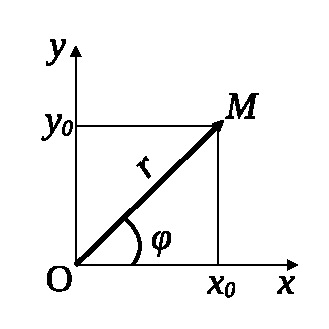
\includegraphics[width=0.33\textwidth]{images/img1}
    \caption{Изображение числа \(z\) на плоскости}
    \label{img1}
\end{figure}
\tcchapter{Решение и разбор задач с применением метода}
\section*{Задача 1}
\paragraph{Постановка задачи:}
Доказать, что если некоторая прямая пересекает прямые, содержащие стороны \(BC\), \(CA\), \(AB\) треугольника \(ABC\), в точках \(A_1\) , \(B_1\) , \(C_1\) соответственно, то середины отрезков \(AA_1\) , \(BB_1\) , \(CC_1\) коллинеарны.
\begin{figure}[h]
    \centering
    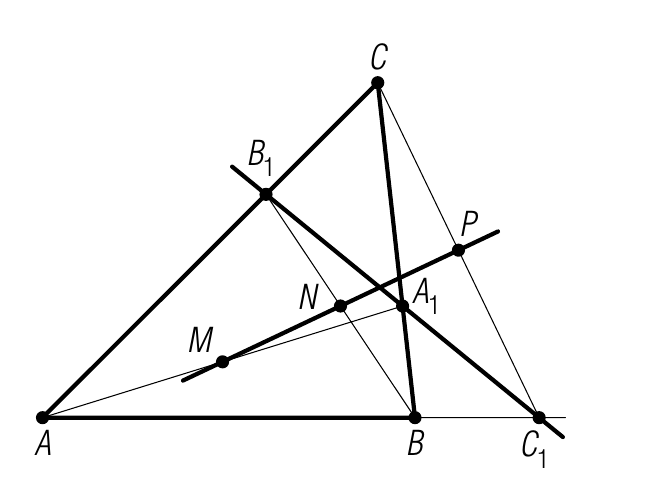
\includegraphics[width=0.5\textwidth]{images/task1.png}
    \caption{Иллюстрация к задаче}
    \label{task1}
\end{figure}
\paragraph{Решение задачи:}
%FIXME Для решения данной задачи требуется найти достаточные критерии коллинеарности точек 3 точек.
Условие коллинеарности троек точек \(A, B_1 , C\); \(C,
A_1 , B\); \(B, C_1 , A\); \(A_1 , B_1 , C_1\):

\begin{equation}
    \left\{ \begin{aligned}
         & a(\bar{b_1} - \bar{c}) + b_1(\bar{c} - \bar{a}) + c(\bar{a} - \bar{b_1}) = 0             \\
         & b(\bar{c_1} - \bar{a}) + c_1(\bar{a} - \bar{b}) + a(\bar{b} - \bar{c_1}) = 0             \\
         & c(\bar{a_1} - \bar{b}) + a_1(\bar{b} - \bar{c}) + b(\bar{c} - \bar{a_1}) = 0             \\
         & a_1(\bar{b_1} - \bar{a_1}) + b_1(\bar{a_1} - \bar{a_1}) + a_1(\bar{a_1} - \bar{b_1}) = 0 \\
    \end{aligned}
    \right. \label{form:1}
\end{equation}
Если \(M, N, P\) -- середины отрезков \(AA_1, BB_1, CC_1\), то предстоит показать, что
\begin{equation}
    m(\bar{n} -\bar{p})+n(\bar{p}-\bar{m})+p(\bar{m}-\bar{n})=0,
    \label{form:2}
\end{equation}
Так как \(\displaystyle
m=\frac{1}{2}(a+a_1),\;
n=\frac{1}{2}(b+b_1),\;
p=\frac{1}{2}(c+c_1)
\), то доказываемое равенство (\ref{form:2}) эквивалентно такому:

\(
(a+a_1)(\bar{b}+\bar{b_1}-\bar{c}-\bar{c_1})+(b+b_1 )(\bar{c}+\bar{c_1}-\bar{a}-\bar{a_1})+(c+c_1)(\bar{a}+\bar{a_1}-\bar{b}-\bar{b_1})=0,
\) или, после перемножения,
\begin{equation}
    \begin{aligned}
         & a(\bar{b_1} - \bar{c}) + a(\bar{b}- \bar{c_1}) + a_1(\bar{b_1} - \bar{c_1}) + a_1(\bar{b}- \bar{c}) + b(\bar{c_1} - \bar{a}) + b(\bar{c}- \bar{a_1}) + \\
         & +b_1(\bar{c_1}-\bar{a_1})+b_1 (\bar{c}-\bar{a})+c(\bar{a_1}-\bar{b})+c(\bar{a}-\bar{b_1})+c_1 (\bar{a_1}-\bar{b_1} )+c_1(\bar{a}-\bar{b})=0.
    \end{aligned}
    \label{form:3}
\end{equation}
Теперь легко видеть, что (\ref{form:3}) получается при почленном сложении
равенств (\ref{form:1})
\paragraph*{Алгоритм программного решения частного случая задачи:} На вход программы передаются координаты свободных точек комплексной плоскости, в данном примере это координаты точек \(A,B,C,A_1,B_1\). Если \(A_1,B_1\) лежат на треугольнике, то по данным входным данным строится прямая, соответствующая условиям задачи. Далее производится проверка того, что середины отрезков \(AA_1,BB_1,CC_1\) коллинеарны. Если условие выполняется,то задача считается решенной для данных входных данных и на экран выводятся координаты точек \(M,N,P\), а также координаты всех остальных. Блок-схема алгоритма приведена на Рис. \ref{task1-scheme}.
\begin{center}
    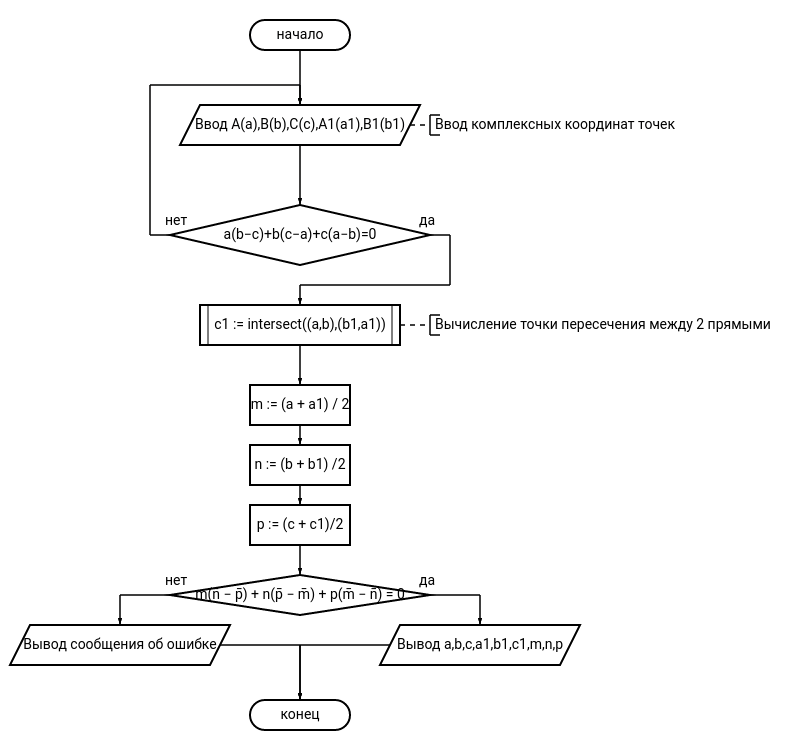
\includegraphics[width=0.9\textwidth]{images/diagram-1.png}
    \captionof{figure}{Блок-схема алгоритма программы}
    \label{task1-scheme}
\end{center}

\paragraph*{Программная реализация задачи:} Решение задачи написано на языке C++ в как часть программы для решения задач из данной работы.
Реализация алгоритма программы предоставлена в функции task1 (файл \filename{\taskFileName{1}}):
\lstinputlisting[frame=none,caption={Функция task1},label=task1-code,captionpos=b,firstline=3]{\taskFileName{1}}

\paragraph*{Демонстрация работы:}
Здесь будут скриншоты работы.

\section*{Задача 2}
\paragraph{Постановка задачи:} Показать, что ортогональные
проекции точки, лежащей на описанной около
треугольника окружности, на прямые, содержащие его стороны, коллинеарны.
\begin{figure}[ht]
    \centering
    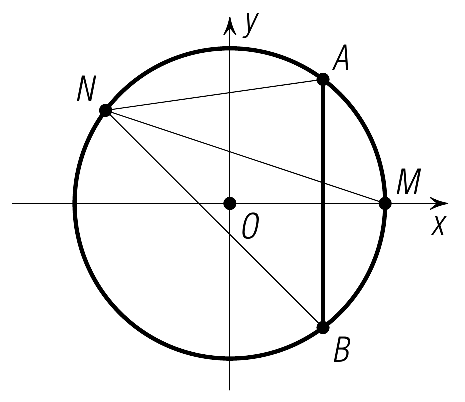
\includegraphics[width=0.5\textwidth]{images/task2.png}
    \caption{Иллюстрация к задаче}
    \label{task2}
\end{figure}
\paragraph{Решение задачи:}
За центр окружности примем точку O

\section*{Задача 3}
\tcchapter{Заключение}
В ходе выполнения работы изложены основы метода комплексных чисел, было проиллюстрировано его применение при решении 3 задач. Каждая задача имеет решение на языке C++.


Таким образом, все поставленные задачи были успешно выполнены, цель
достигнута.
%bibliography
\renewcommand\bibname{Список литературы}
\begin{thebibliography}{00}
   \addcontentsline{toc}{chapter}{Список литературы}
   \bibitem{book:ponarin} Понарин~Я.П. Алгебра комплексных чисел в геометрических задачах:
   Книга для учащихся математических классов школ, учителей и студентов педагогических вузов. --~М.:~МЦНМО,
   2004. -- 160 с.
   \bibitem{book:takeuti} Такеути Г. Теория доказательств. -- Пер. с англ. --~М.:~Мир, 1978. -- 414 с.
   \bibitem{book:sloyer} Слойер К. Математические фантазии. -- Пер. с англ. --~М.:~Мир, 1993. -- 184 с.
   \bibitem{book:kosnevsky} Коснёвски Ч. Занимательная математика и персональный компьютер. -- Пер. с англ. --~М.:~Мир, 1987. -- 192 c.
   \bibitem{geom:methods} Кибирев~В.~В. Обучение методам решения геометрических задач // Вестник~БГУ.~2014.~№15. URL:~\href{https://cyberleninka.ru/article/n/obuchenie-metodam-resheniya-geometricheskih-zadach}{https://cyberleninka.ru/article/n/obuchenie-metodam-resheniya-geometricheskih-zadach} (дата обращения:~19.07.2022).
   \bibitem{book:semendyaev} Бронштейн~И.~Н., Семендяев~К.~А. Справочник по математике для инженеров и учащихся втузов.-- 13-е изд., исправленное. --~М.:~Наука, Гл.~ред.~физ.-мат.~лит., 1986. -- 544 с.
   \bibitem{book:arnold_complex} Арнольд~В.~И.Геометрия комплексных чисел, кватернионов и спинов. -- 4-е изд., стереотипное. --~М.:~МЦНМО, 2014. -- 40 с.
   \bibitem{book:jaglom} Яглом~И.~М., Семендяев~К.~А. Комплексные числа и их применения в геометрии.-- 2-е изд., стереотипное. --~М.:~Едиториал~УРСС, 2004. -- 192 с.
   \bibitem{edu:problem} Жмурова~И.~Ю. Изучение комплексных чисел в общеобразовательной школе / И.~Ю.~Жмурова, С.~В.~Баринова. // Молодой~ученый. -- 2020. -- №~5~(295). -- С.~312-314. -- URL:~\href{https://moluch.ru/archive/295/67123/}{https://moluch.ru/archive/295/67123/} (дата обращения: 17.05.2022).
\end{thebibliography}


\end{document}
